

\section{Thales}
\subsection{System architecture}
\frame
{
  \frametitle{Thales System architecture}
 \begin{center}
	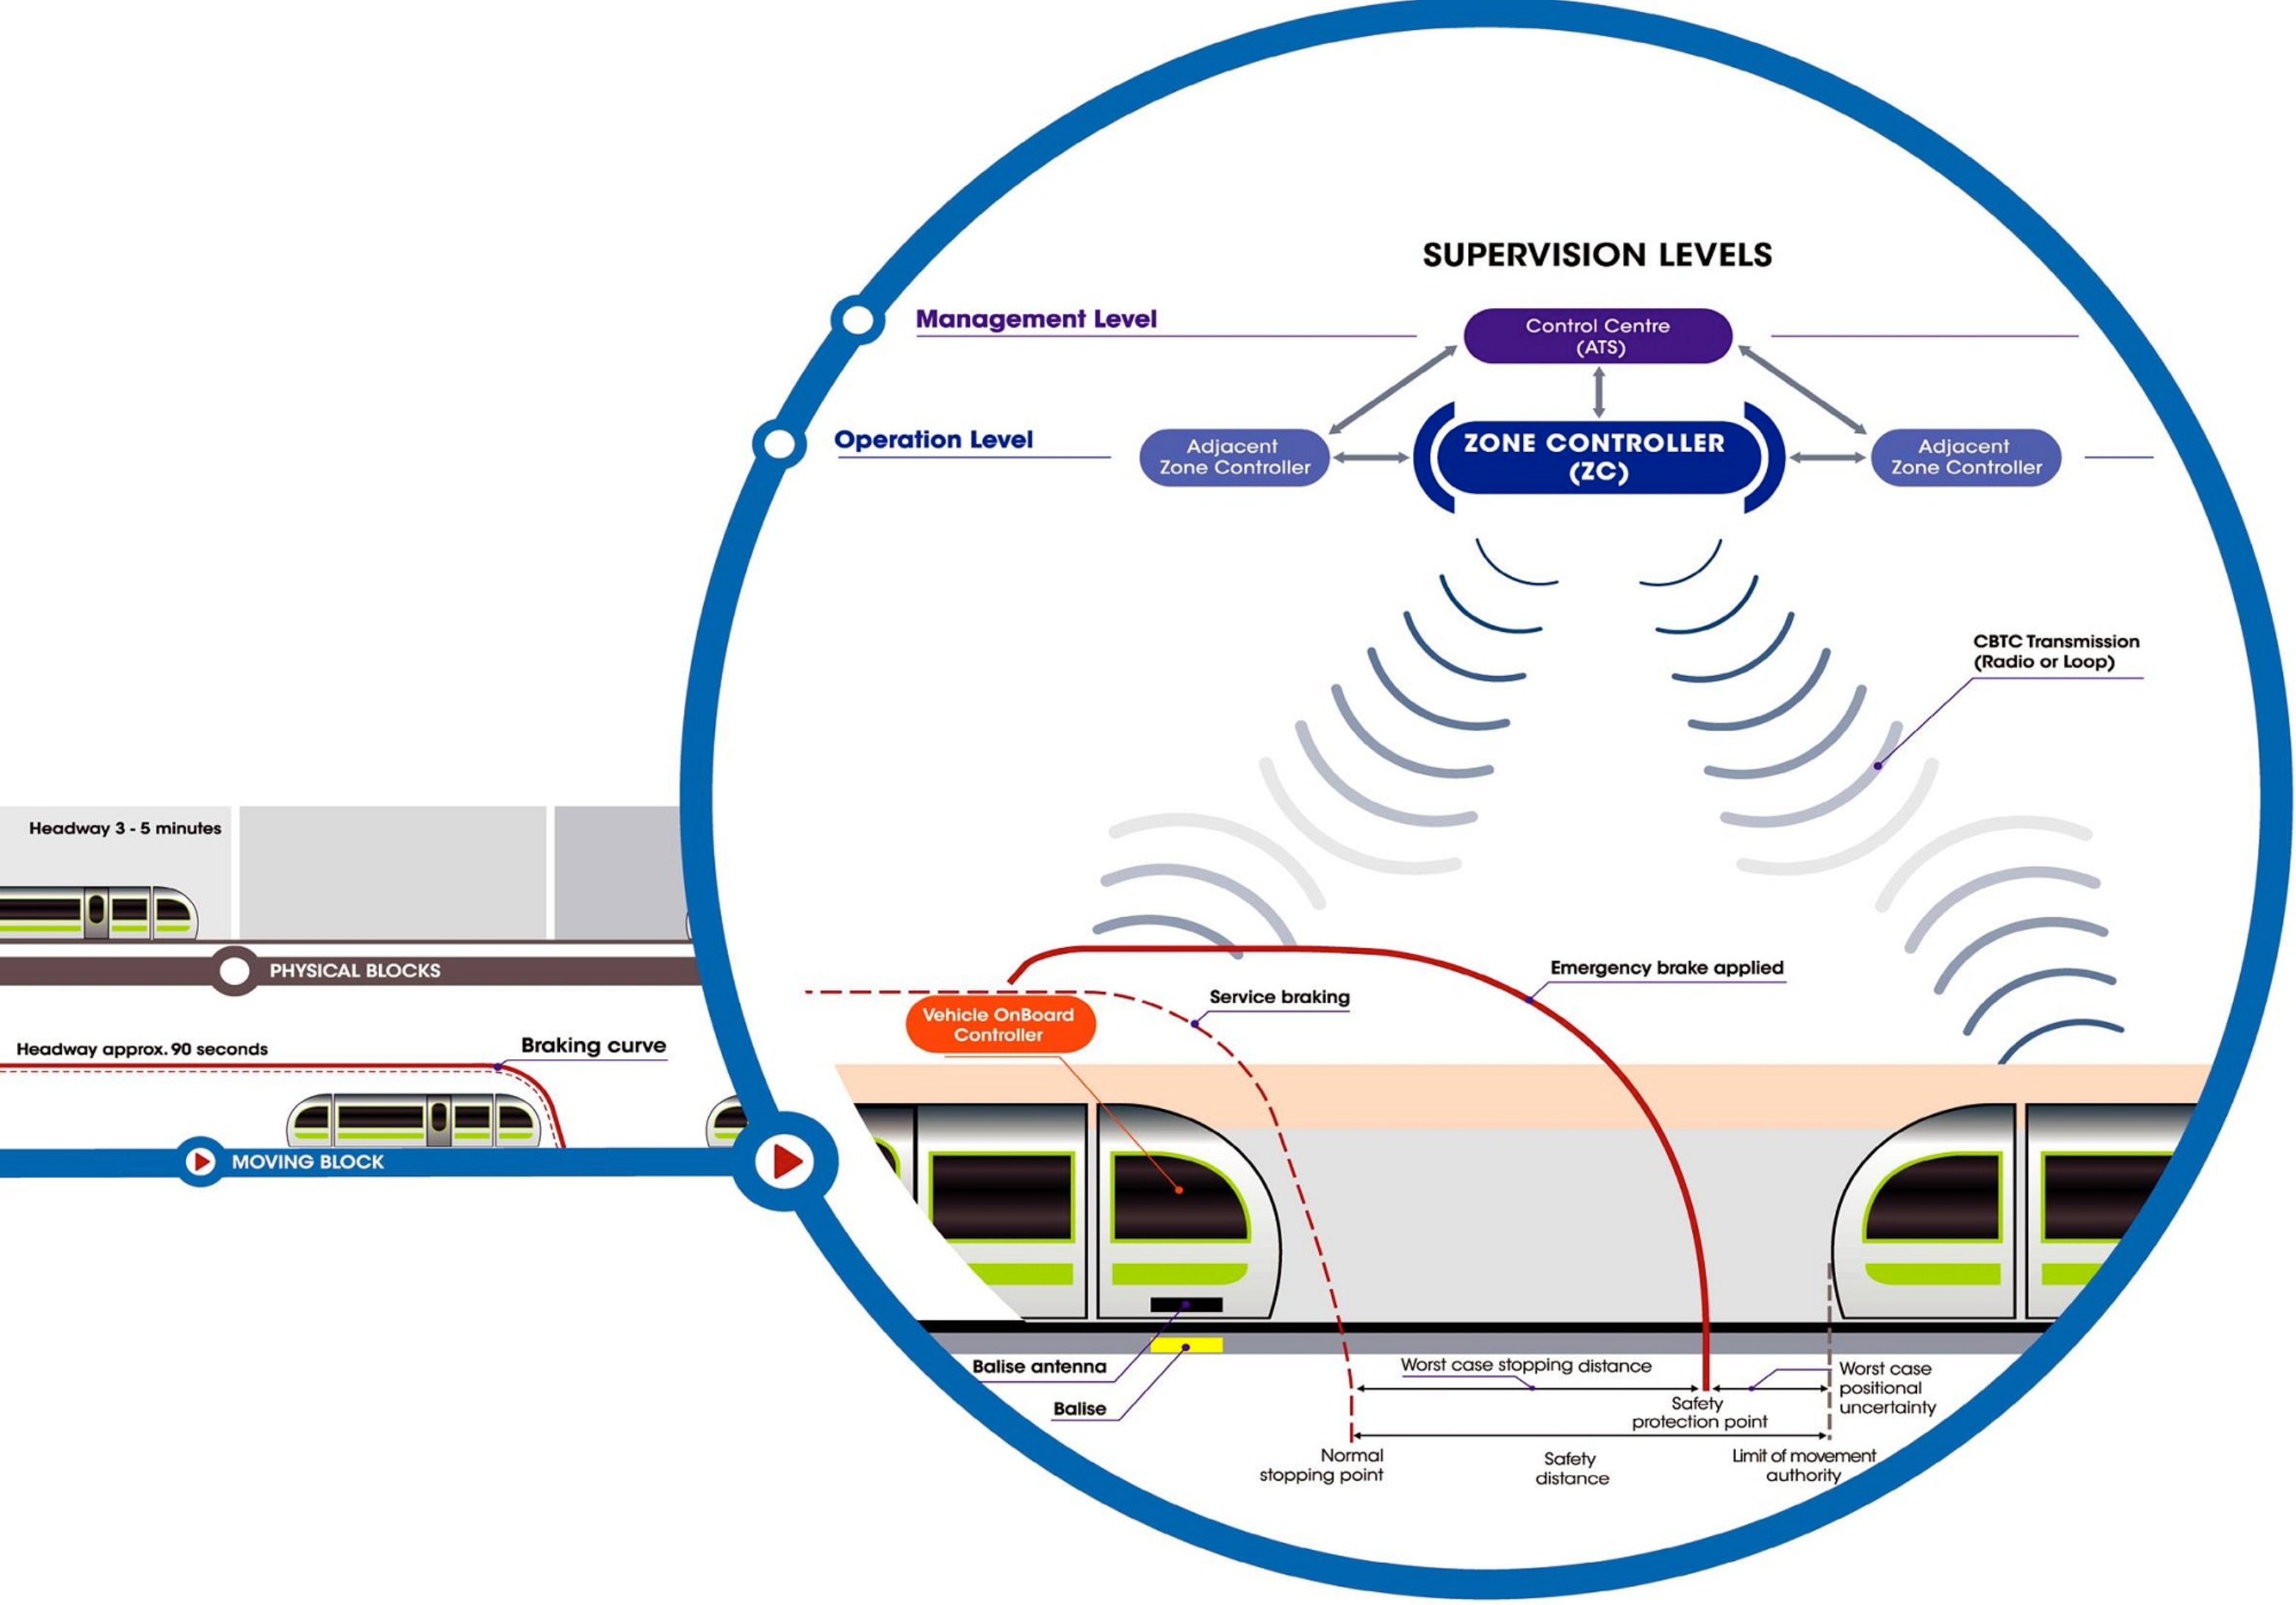
\includegraphics[scale=0.2]{./fig/SeltracArchitetture2}
      \end{center}
   
}

\frame
{
  \frametitle{Thales System architecture Loop Inductive Version}
 \begin{center}
	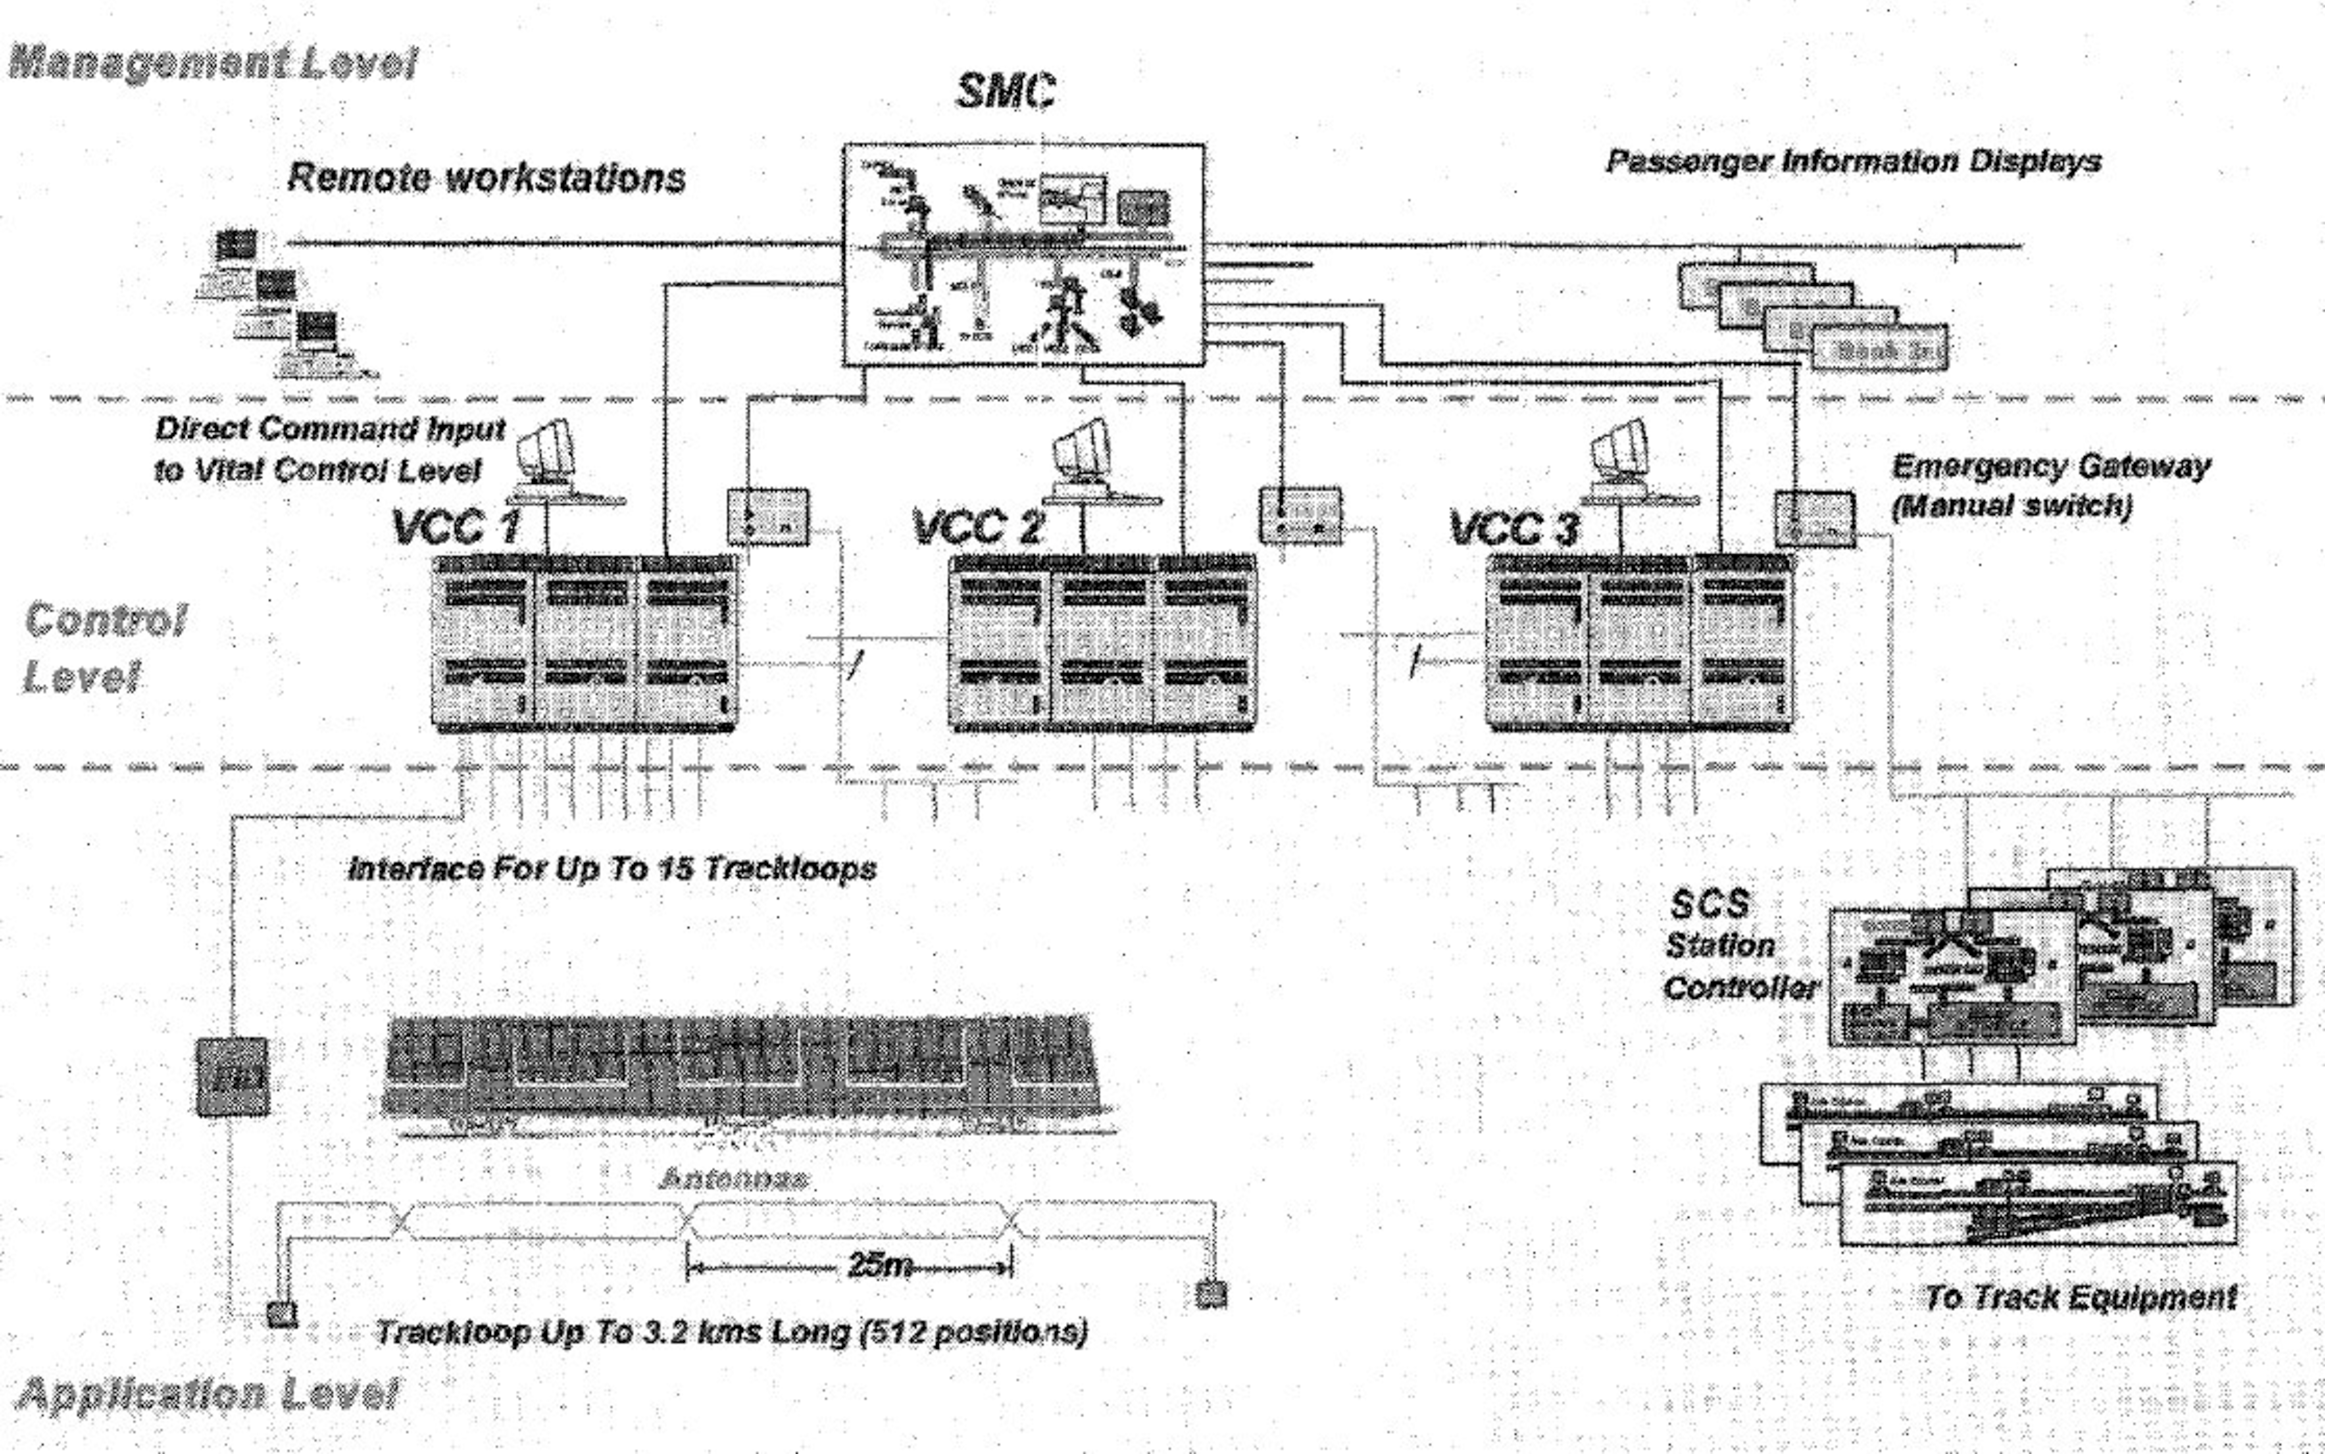
\includegraphics[scale=0.25]{./fig/SeltracTBTCArchitetture}
      \end{center}
      {\tiny  SMC is Supervisory Control Level, VCC is Vehicle Control Computer, SCS is Station Controller Systems}
   
}

\frame
{
  \frametitle{Thales System architecture Radio Frequency Version}
 \begin{center}
	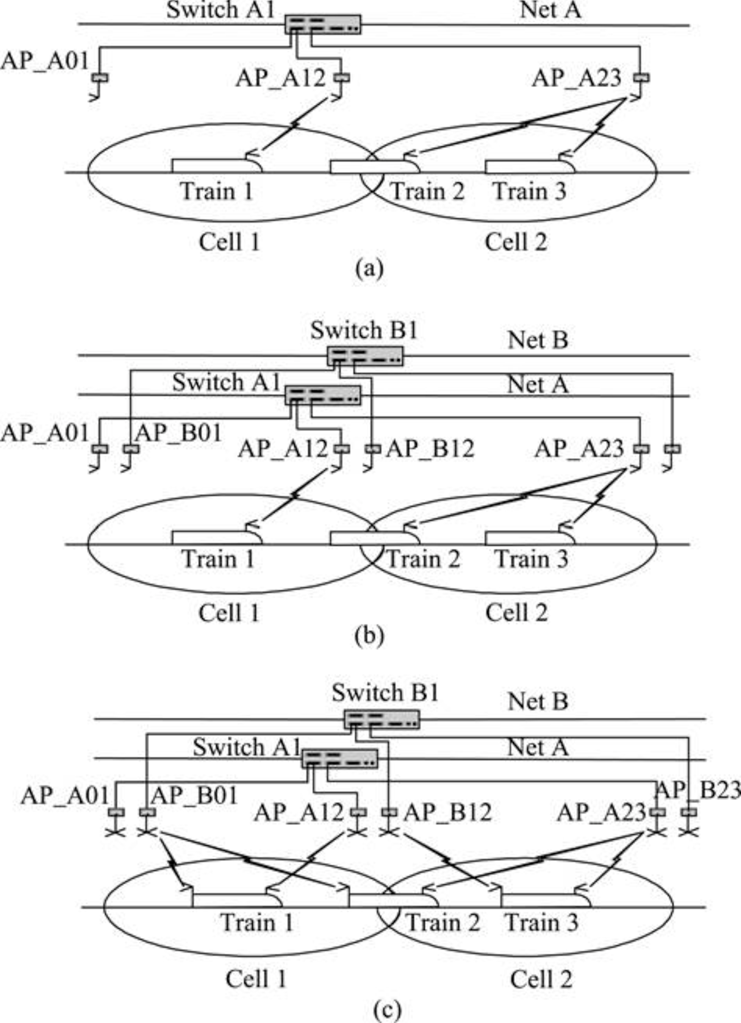
\includegraphics[scale=0.45]{./fig/SeltracRFArchitetture}
      \end{center}
      
   
}

\subsection{Operating mode, Safety and failure management}
\frame
{
\begin{block}<1->{Operating mode management}
Replacing or overlay existing signalling
\end{block}
\begin{alertblock}<2->{Safety and failure management}
Seltrac S40 uses fully redundant computer systems 

   \end{alertblock}
}


\subsection{Communication infrastructure and protocol }
\frame
{
  
\begin{block}<1->{Communication infrastructure and protocol}
\begin{itemize}
\item IL \begin{itemize}
\item Train-wayside protocol is Proprietary.  VOBC antennas to receive data at 36 kHz and to transmit data at 56 kHz.  The protocol used in Alcatel's loop communication has the VCC transmitting an 83-bit telegram to the VOBC at 1200 baud; the VOBC responds with a 43 bit telegram at 600 baud.  

\end{itemize}

\item RF \begin{itemize}
\item system are fully redundant.
\item Train-wayside protocol : IEEE 802.11
\item On Board Communication sub-system has two antennas, one on the front, and one on the rear of the train. Each onboard network device connected to the antenna is a modular component, with two IEEE 802.3 interfaces, as well as one CAN bus interface.
\end{itemize}


\end{itemize}

     




\end{block}


}

%System architecture
%Operating mode management
%Safety and failure management
%Communication infrastructure and protocol
%Interlocking and wayside information integration

\subsection{ATS functions}
\frame
{

\begin{block}<1->{Interlocking and wayside information integration}
The interlocking functions are provided by LockTrac 6131 ELEKTRA is an electronic interlocking system that provides the highest levels of safety and availability.


   \end{block}
  
\begin{block}<2->{ATS functions}
\begin{itemize}
\item Train departure, destination assignments and identification assignment.
\item Train routing functions.
\item Modification of the system operations parameters in response to system delays and Control Room commands.
\item Data logging.
\item Station platform information display (PID) control
\item Station platform announce
\end{itemize}
\end{block}
}


%ATS functions

\subsection{Headway,  }
\frame
{
  

\begin{block}<1->{Headway and Braking model}
\begin{itemize}
\item SelTrac has proven that it can deliver headways of under 60s. 
\item In Dubai Metro is configured for a minimum headway of 90s.

 
\end{itemize}

   \end{block}
   
   \begin{block}<2->{Braking models and speed limit protection}
The system allows four service brake rates ranging from 0.4$ms^{-2}$ to 0.8$ms^{-2}$.  

The brake rate for a specific train or track section can be adjusted manually from the control center.

Safety calculations are based on an emergency brake rate of 0.9$ms^{-2}$

   \end{block}
   
     }

%Headway
%Braking models and speed limit protection
%Train speed and train location determination

\subsection{Train speed, train location determination,Door management, ATO functions}
\frame
{
   \begin{block}<1->{Train speed and train location determination}
      \begin{itemize}
       \item With IL for speed determination use a tacho-generators, used to measure speed, direction and distance in conjunction with an accelerometer. SELTRAC train position detection system provides a 6.25 meter resolution.

\item With radio-based the system use the trackside transponder tags assist in train positioning

\item Maximum speed of the trains will be 90 km/h.

\end{itemize}



   \end{block}


\begin{block}<2->{Door management}
No Information

   \end{block}
   
   \begin{block}<3->{ATO functions}
  Control train movement with regard to speed, acceleration, deceleration, and jerk.
   \end{block}
   
   }


%Door management
%ATO functions

\subsection{Service-oriented facilities}
\frame
{  
   
      \begin{block}<1->{Service-oriented facilities}
      \begin{itemize}
       \item Passenger information displays (PIDs)
\item CCTV surveillance
\item Public announcement (PA)
\item Audio and video recording
\item Phone system and emergency
\item Advertising information system audio / video
\item Supervisory Control and Data Acquisition (SCADA) 
\item Emergency call points allow direct communication with passengers from centralised Operational control centre.
\item Access control: used to detect and warn in the event of unauthorised access to particular areas of the network
\end{itemize}



   \end{block}
   
    \begin{block}<2->{}
   End
   \end{block}
}

%Service-oriented facilities
%qui
  %\begin{itemize}
  %\item<1-> Normal LaTeX class.
  %\item<2-> Easy overlays.
  %\item<3-> No external programs needed.      
  %\end{itemize}

